

Suponhamos um estado inicial $t_1$ da seguinte maneira (vamos suprimir as informações sobre mãos e baralhos pois estas são irrelevantes)

\vskip1ex

\textbf{Figura E.2.1:} estado $t_1$

\begin{mdframed}
    \begin{center}
    $t_1 = \left\{ v_1 = v_2 = 10, G_1 = G_2 = \emptyset, B_1, B_2 \right\}$
    \vskip1ex
    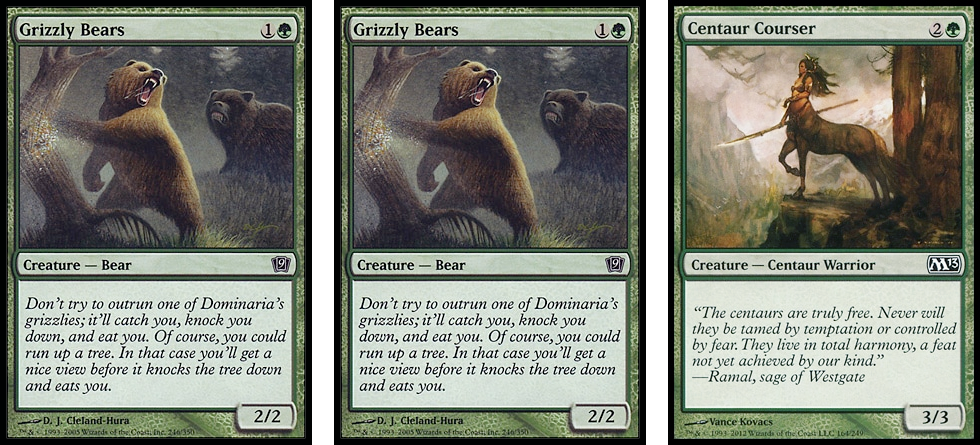
\includegraphics[width=0.5\textwidth]{picstcc/att1.png}
    \vskip1ex
    $B_1$: O jogador ativo tem três criaturas aptas a atacar em campo: dois ``Grizzly Bears'' e um ``Centaur Courser''. Assim, podemos obter o conjunto de ações legais $A^C_1$:

    \begin{equation}
      A^C_1(t_{1,1}) := \begin{lrdcases}
                  GrizzlyBears1, \\
                  GrizzlyBears2, \\
                  CentaurCourser, \\
                  \{ GrizzlyBears1, GrizzlyBears2\}, \\
                  \{ GrizzlyBears1, CentaurCourser \}, \\
                  \{GrizzlyBears2, CentaurCourser \}, \\
                  \{ GrizzlyBears1, GrizzlyBears2, CentaurCourser\}, \\
                  None.
                  \end{lrdcases}
    \end{equation}
    O jogador ativo pode declarar qualquer combinação (incluindo nenhuma) de criaturas como atacantes. Note que $N = 3$ e $|A^C_1| = 2^N = 8$.
  \end{center}
\end{mdframed}

Suponhamos que o jogador ativo escolheu a ação $\{GrizzlyBears2, CentaurCourser\}$ em $t_1$. Assim, o jogador declarou ambas suas criaturas como atacantes. Assim como com terrenos e geração de recursos, uma criatura atacante é virada quando declarada atacante (e precisa estar desvirada previamente para poder atacar). Assim, podemos obter o estado seguinte, $t_2$.

\newpage

\textbf{Figura E.2.2:} estado $t_2$

\begin{mdframed}
    \begin{center}
    $t_2 = \left\{ v_1 = v_2 = 10, G_1 = G_2 = \emptyset, B_1, B_2 \right\}$\\
    $R(t_2) = \frac{10-10}{5} + (7 - 4) + \frac{7-4}{2} = 4,5$
    \vskip1ex
    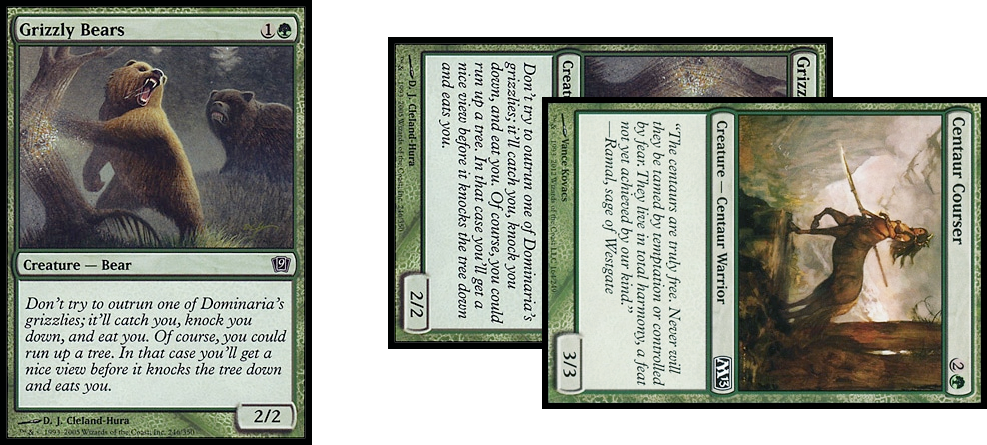
\includegraphics[width=0.5\textwidth]{picstcc/att2.png}
    \vskip1ex
    $B_1$: O jogador ativo tem um ``Grizzly Bears'' desvirado e um ``Grizzly Bears'' e um ``Centaur Courser'' virados, ambos atacando ($N' = 2$).

    \vskip1ex

    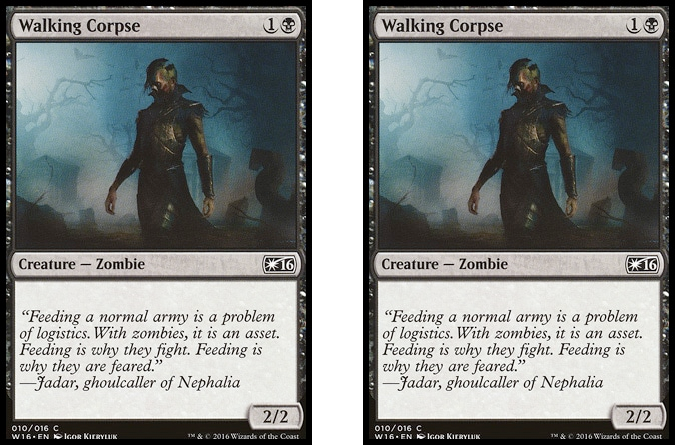
\includegraphics[width=0.4\textwidth]{picstcc/blk1.png}

    \vskip1ex
    $B_2$: O jogador defensor tem dois ``Walking Corpse'' desvirados (e aptos a bloquear). Portanto, as ações legais são todas as combinações de bloqueio das criaturas atacantes:

    \begin{equation}
      A^C_2(t_2) := \begin{lrdcases}
                  \{WalkingCorpse1 : None, WalkingCorpse2 : None\}, \\
                    \{WalkingCorpse1 : GrizzlyBears2, WalkingCorpse2 : None\}, \\
                  \{WalkingCorpse1 : CentaurCourser, WalkingCorpse2 : None\}, \\
                  \{WalkingCorpse1 : None, WalkingCorpse2 : GrizzlyBears2\}, \\
                  \{WalkingCorpse1 : None, WalkingCorpse2 : CentaurCourser\}, \\
                  \{WalkingCorpse1 : CentaurCourser, WalkingCorpse2 : GrizzlyBears2\}, \\
                  \{WalkingCorpse1 : GrizzlyBears2, WalkingCorpse2 : CentaurCourser\}, \\
                  \{WalkingCorpse1 : GrizzlyBears2, WalkingCorpse2 : GrizzlyBears2\}, \\
                  \{WalkingCorpse1 : CentaurCourser, WalkingCorpse2 : CentaurCourser\}.
                  \end{lrdcases}
    \end{equation}
    Assim, há $|A^C_2(t_2)| = (N' + 1)^M = (2 + 1)^2 = 9$ ações legais.
  \end{center}
\end{mdframed}

Assim, há alguns estados sucessores possíveis. Vamos examinar algumas configurações de bloqueio distintas\footnote{Algumas ações são essencialmente a mesma, pois os dois ``Walking Corpse'' não têm diferenças. Como, nas regras do jogo, são considerados objetos diferentes, estamos distinguindo-os para manter a consistência.} e seus respectivos estados sucessores.

\newpage

\textbf{Figura E.2.3:} estado $t_3$

\begin{mdframed}

    Suponhamos que a ação escolhida pelo agente tenha sido \[\{WalkingCorpse1 : GrizzlyBears2, WalkingCorpse2 : None\},\] ou seja, bloquear ``Grizzly Bears'' com um ``Walking Corpse'' e não bloquear ``Centaur Courser''.

    \begin{center}
    \vskip1ex
    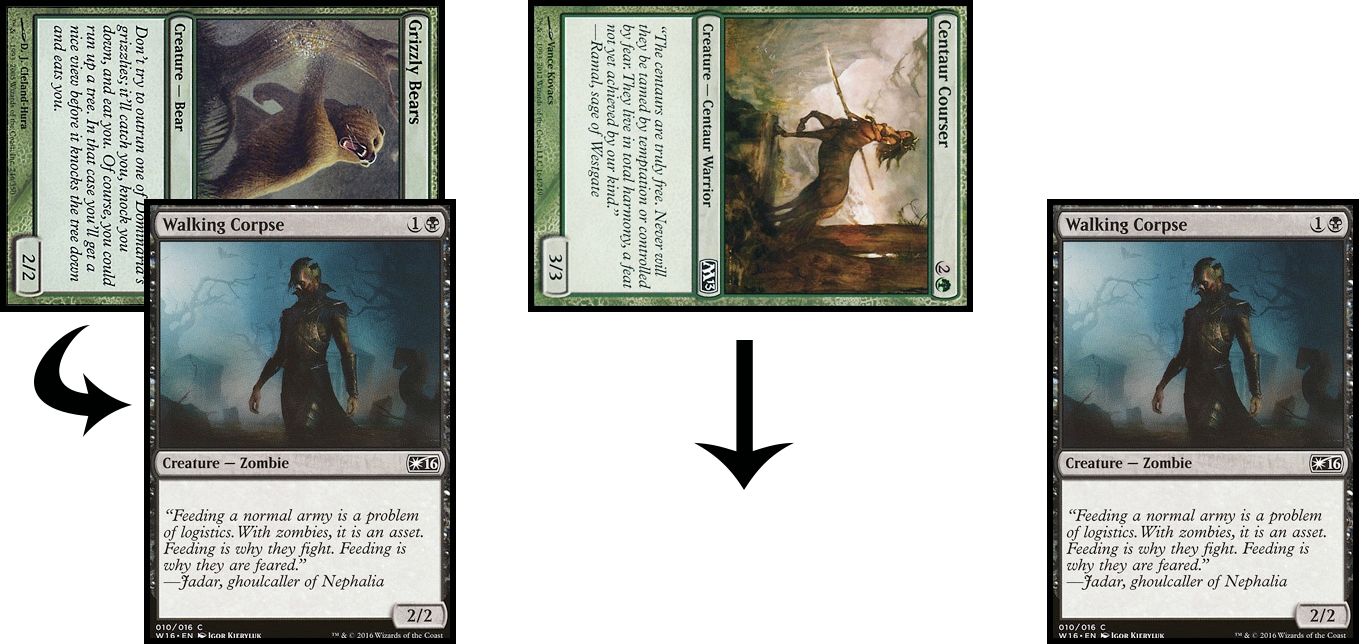
\includegraphics[width=0.9\textwidth]{picstcc/blk2.png}
    \vskip1ex
    Esta é a representação da ``resolução do combate'' pré-$t_3$. O estado $t_3$, portanto, refletirá as consequências das ações escolhidas. Podemos listá-las:
    \begin{itemize}
      \item ``Grizzly Bears'' causou um número igual a seu poder (2) de dano ao ``Walking Corpse'' que o bloqueou.
      \item ``Walking Corpse'' causou um número igual a seu poder (2) de dano ao ``Grizzly Bears'' bloqueado.
      \item ``Centaur Courser'' não foi bloqueado, causando um número igual a seu poder (3) de dano ao jogador defensor.
    \end{itemize}
    \end{center}

    Assim, ambos ``Grizzly Bear'' e ``Walking Corpse'' são destruídos (pois receberam dano maior ou igual às suas resistências) e temos o seguinte estado $t_3$:

    \[t_3 = \begin{lrdcases}
           v_1 = 10, v_2 = 10 - 3 = 7, \\
           G_1 = \{ GrizzlyBears2 \}, G_2 = \{ WalkingCorpse1 \}, \\
           B_1 = \{ GrizzlyBears1(u), CentaurCourser(t)\}, \\
           B_2 = \{ WalkingCorpse2(u) \}.
           \end{lrdcases}\]
    \begin{equation*}
      R(t_3) = \frac{7}{5} + (5-2) + \frac{5-2}{2} = 5,9
    \end{equation*}
    O parâmetro $u$ de uma permanente significa que ela está desvirada, enquanto $t$ significa que está virada.
\end{mdframed}

Em $t_3$, ambos os jogadores tem uma criatura (essencialmente igual, pois têm os mesmos atributos) a menos em relaçnao a $t_2$, mas o jogador defensor perdeu pontos de vida.

\pagebreak

\textbf{Figura E.2.4:} estado $t'_3$

\begin{mdframed}

    Suponhamos, por outro lado, que a ação escolhida pelo agente tenha sido \[\{WalkingCorpse1 : GrizzlyBears2, WalkingCorpse2 : CentaurCourser\},\] ou seja, bloquear ``Grizzly Bears'' com um ``Walking Corpse'' e ``Centaur Courser'' com o outro.

    \begin{center}
    \vskip1ex
    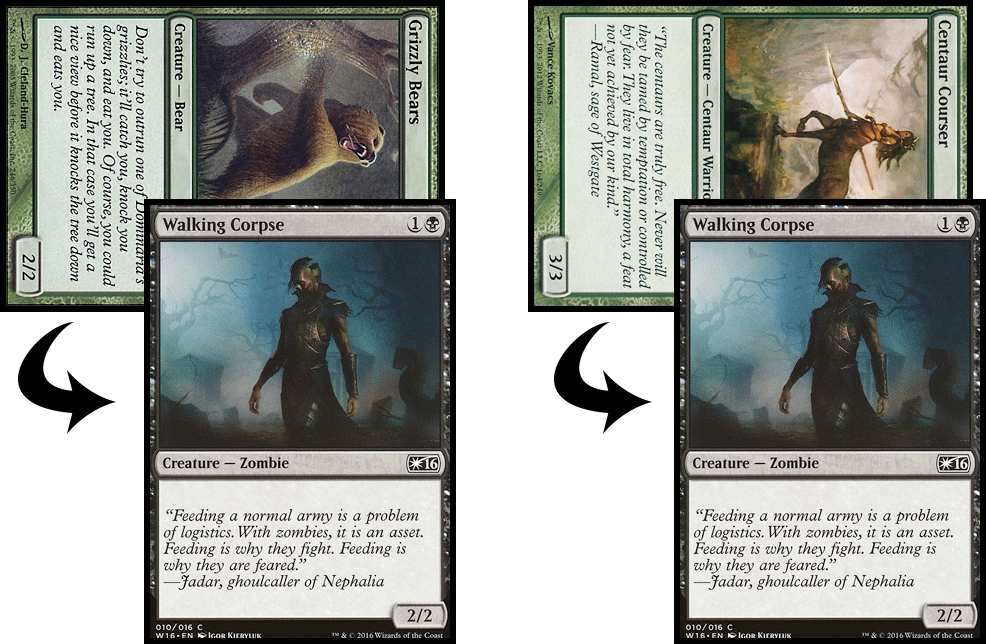
\includegraphics[width=0.9\textwidth]{picstcc/blk3.png}
    \vskip1ex
    Representação do combate. O estado $t'_3$ refletirá as seguintes consequências:
    \begin{itemize}
      \item ``Grizzly Bears'' causou um número igual a seu poder (2) de dano ao ``Walking Corpse'' que o bloqueou.
      \item ``Walking Corpse'' causou um número igual a seu poder (2) de dano ao ``Grizzly Bears'' bloqueado.
      \item ``Centaur Courser'' causou um número igual a seu poder (3) de dano ao ``Walking Corpse'' que o bloqueou.
      \item ``Walking Corpse'' causou um número igual a seu poder (2) de dano ao ``Centaur Corser'' bloqueado.
    \end{itemize}
    \end{center}

    Assim, ``Grizzly Bears'' e os dois ``Walking Corpse'' são destruídos (pois receberam dano maior ou igual às suas resistências) e temos o seguinte estado $t'_3$:

    \[t'_3 = \begin{lrdcases}
           v_1 = 10, v_2 = 10, \\
           G_1 = \{ GrizzlyBears2 \}, G_2 = \{ WalkingCorpse1, WalkingCorpse2 \}, \\
           B_1 = \{ GrizzlyBears1(u), CentaurCourser(t)\}, \\
           B_2 = \emptyset.
           \end{lrdcases}\]
    \begin{equation*}
      R(t'_3) = \frac{10-10}{5} + (5) + \frac{5}{2} = 7,5
    \end{equation*}
\end{mdframed}

Em $t'_3$, o total de pontos de vida não foi alterado, mas a balança do combate também parece negativa para o jogador defensor, que acabou sem criaturas na mesa. Note que o dano causado a ``Centaur Courser'' não foi suficiente para destruí-lo\footnote{De acordo com as regras, o dano causado a uma criatura permanece até o final do turno. Se, porventura, algum dano fosse causado a ``Centaur Courser'' na segunda fase principal, a criatura também seria destruída.}.

\textbf{Figura E.2.5:} estado $t''_3$

\begin{mdframed}

    Por fim, suponhamos que a ação escolhida pelo agente tenha sido \[\{WalkingCorpse1 : CentaurCourser, WalkingCorpse2 : CentaurCourser\},\] ou seja, bloquear ``Centaur Courser'' com os dois ``Walking Corpse''.

    \begin{center}
    \vskip1ex
    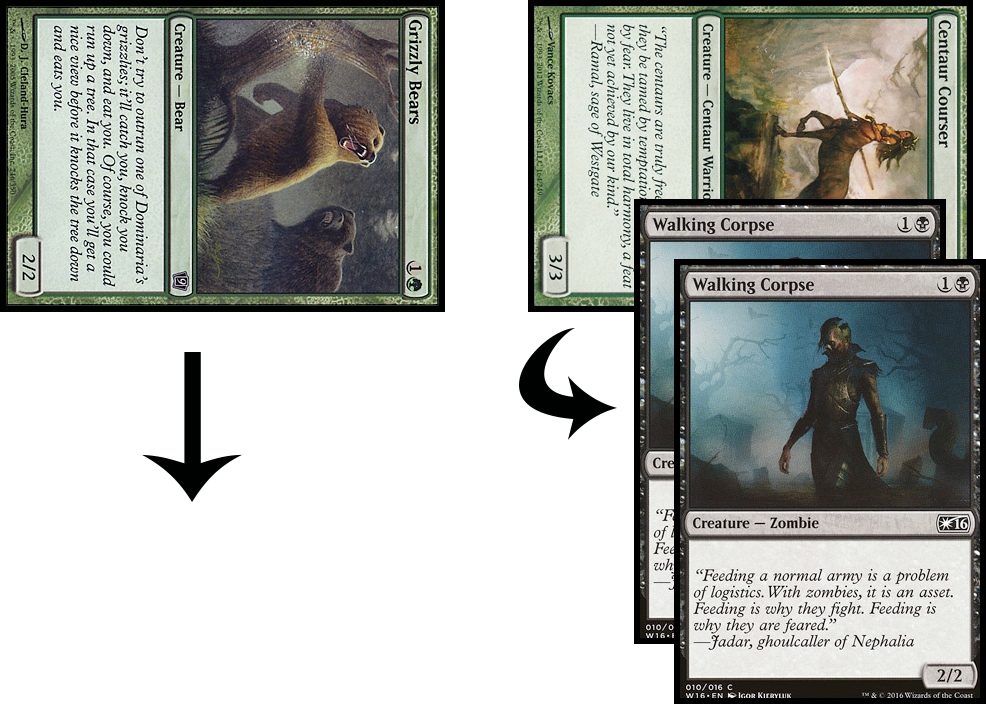
\includegraphics[width=0.9\textwidth]{picstcc/blk4.png}
    \vskip1ex
    Representação do combate. O estado $t''_3$ refletirá as seguintes consequências:
    \begin{itemize}
      \item ``Centaur Courser'' causou um número igual a seu poder (3) de dano aos ``Walking Corpse'' que o bloquearam.
      \item Os dois ``Walking Corpse'' causaram um número igual a seu poder (2 + 2) de dano ao ``Centaur Courser'' bloqueado.
      \item ``Grizzly Bears'' não foi bloqueado, causando um número igual a seu poder (2) de dano ao jogador defensor.
      \item ``Walking Corpse'' causou um número igual a seu poder (2) de dano ao ``Centaur Courser'' bloqueado.
    \end{itemize}
    \end{center}

    Como ``Centaur Courser'' recebeu dano total (4) maior ou igual a sua resistência, foi destruído. Por outro lado, ``Centaur Courser'' causou no total (3) dano suficiente para destruir apenas um ``Walking Corpse'' (e danificar em 1 o outro). O estado $t''_3$, portanto, é configurado assim:

    \[t''_3 = \begin{lrdcases}
           v_1 = 10, v_2 = 10 - 2 = 8, \\
           G_1 = \{ CentaurCourser \}, G_2 = \{ WalkingCorpse1 \}, \\
           B_1 = \{ GrizzlyBears1(u), GrizzlyBears2(t)\}, \\
           B_2 = \{ WalkingCorpse2 \}.
           \end{lrdcases}\]
    \begin{equation*}
      R(t''_3) = \frac{10-8}{5} + (4 -2) + \frac{4-2}{2} = 3,4
    \end{equation*}
\end{mdframed}

Podemos perceber que, para o jogador defensor, a situação é estritamente melhor em $t''_3$ do que em $t_3$, pois $R(t''_3) > R(t_3)$ e, apesar de ter perdido a mesma criatura em ambos os casos, em $t''_3$ o jogador defensor conseguiu destruir uma criatura maior do oponente no processo. Além disso, apesar de não ser estritamente pior, pois não houve perda de vida, a situação em $t'_3$ parece também pior para o jogador defensor do que em $t''_3$, já que acabou perdendo suas duas criaturas.
